\documentclass[a4paper,10pt]{article}
\usepackage[utf8]{inputenc}

\usepackage{graphicx}
\usepackage{float}
\usepackage{amsmath}


% Title Page
\title{Měření krevního tlaku pomocí Honeywell 24PC series senzoru}
\author{Tomáš Kysela}


\begin{document}
\maketitle

\section{Senzor}

\begin{figure}[H]
\centering

\includegraphics[width=0.8\textwidth]{Circuit}
\caption{Schéma zapojení senzoru}
\end{figure}
\begin{figure}[H]
\centering
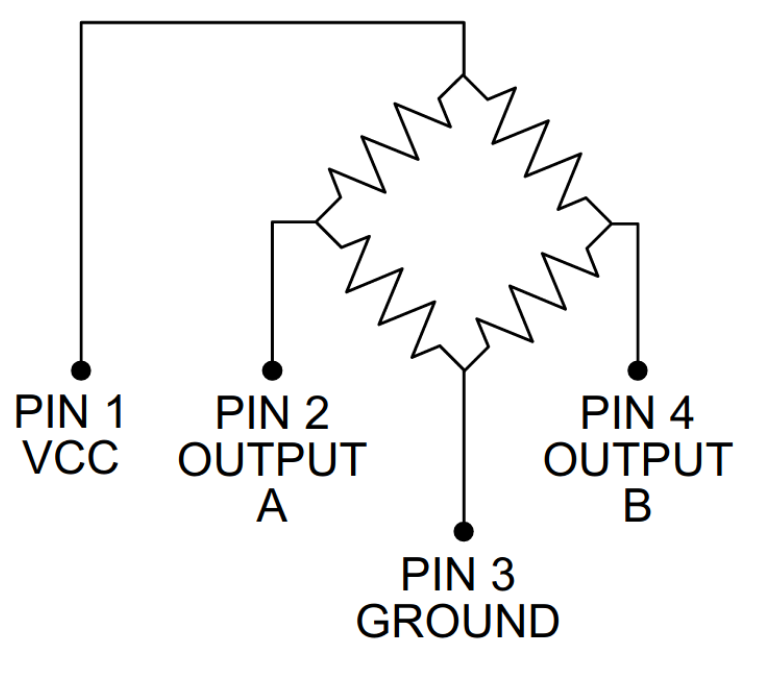
\includegraphics[width=0.8\textwidth]{bridge}
\caption{Vnitřní schéma senzoru}
\end{figure}

\section{Vyhodnovací obvod}

Obovd se dělí na dvě části. Jedna zpracovává DC složku, která určuje tlak v manžetě a AC složku zpracovávající deformace cévy.

\subsection{Tlak v manžetě}
\begin{figure}[H]
\centering
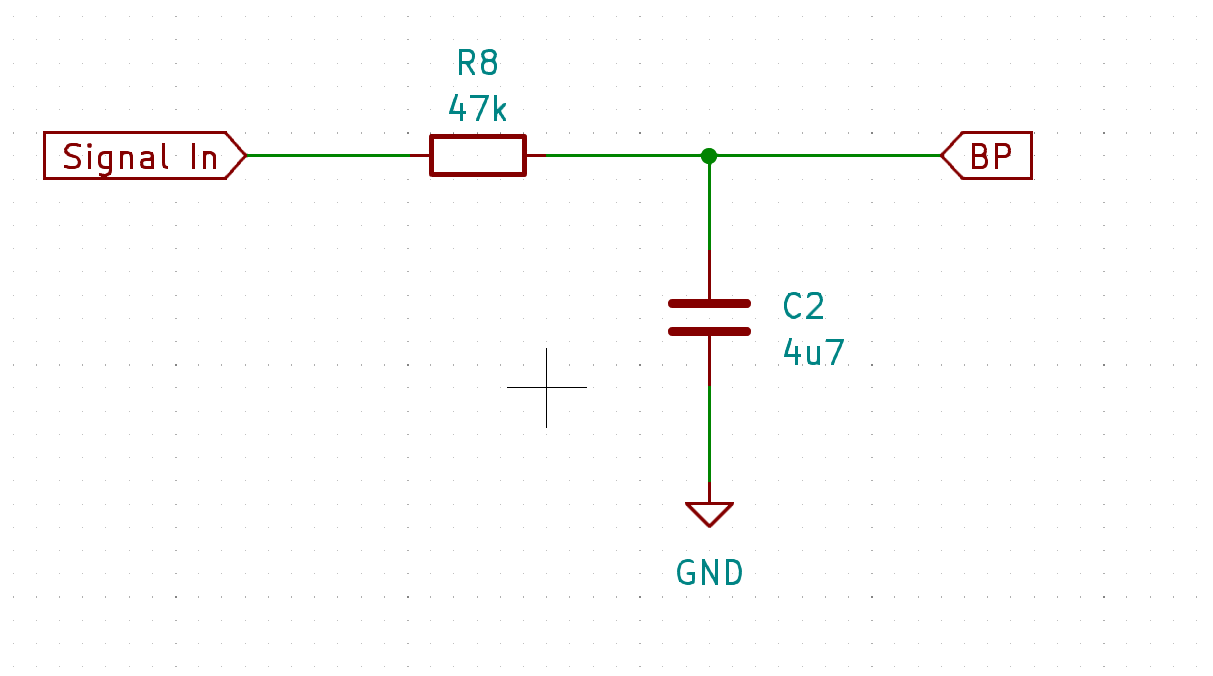
\includegraphics[width=0.8\textwidth]{dc}
\caption{Obvod vyhodnocení DC složky}
\end{figure}
\begin{figure}[H]
\centering
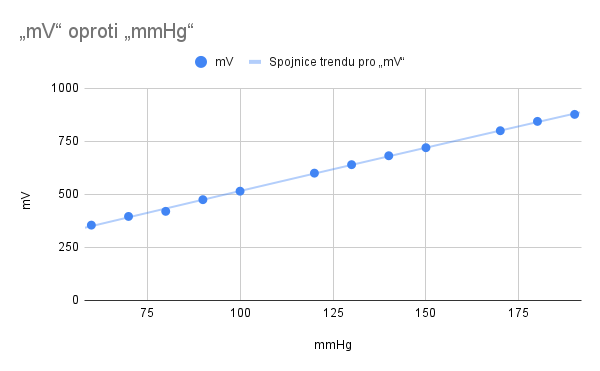
\includegraphics[width=0.8\textwidth]{mmHg}
\caption{Graf vztahu napětí a tlaku}
\end{figure}

Tlak je následně vypočten pomocí vztahu:
\begin{equation}
 P = 2.044185 \cdot U -12.55883
\end{equation}

\subsection{Deformace cévy}

\begin{figure}[H]
\centering
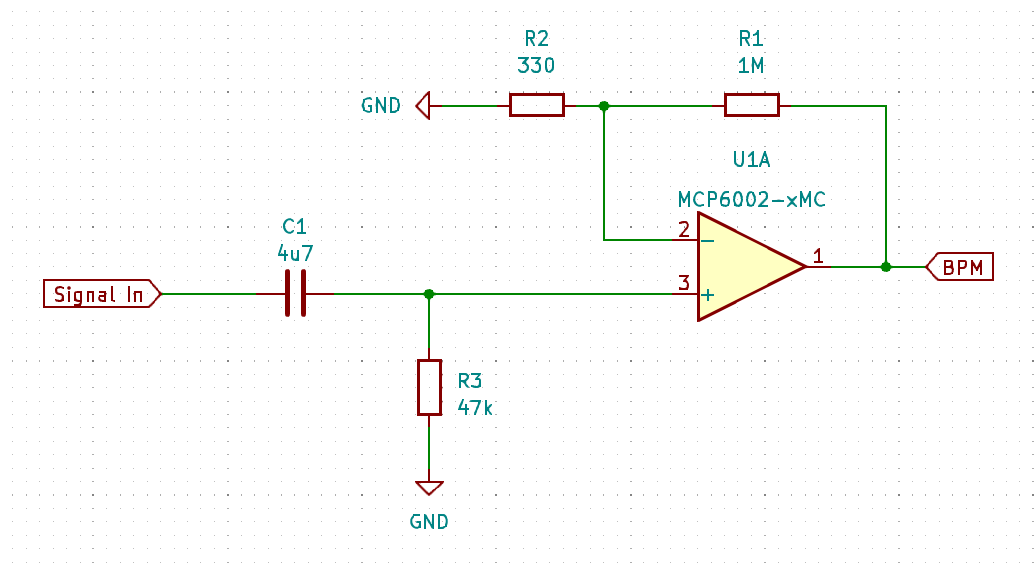
\includegraphics[width=0.8\textwidth]{ac}
\caption{Obvod vyhodnocení AC složky}
\end{figure}
\begin{figure}[H]
\centering
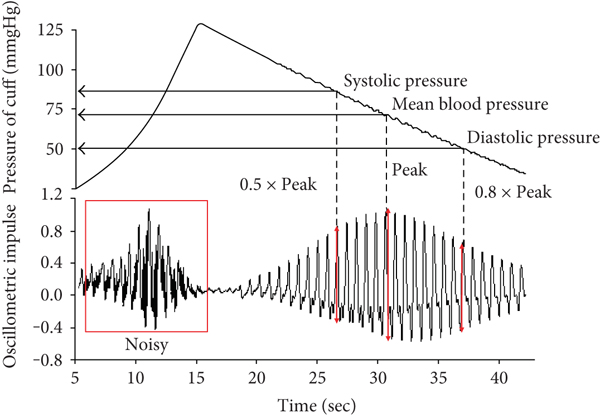
\includegraphics[width=0.8\textwidth]{method}
\caption{Obvod vyhodnocení AC složky}
\end{figure}

Použité konstanty:
\begin{equation}
 SBP = 0.55 \cdot MBP
\end{equation}
\begin{equation}
 DBP = 0.85 \cdot MBP
\end{equation}

\section{Firmware}

Nejdříve je vždy změřena dvojice tlak a amplituda. Pokud je amplituda nad $BPM\_TRASHOLD$, pak je uložena do vektoru. Takto se pokračuje dokud amplituda opět neklesne pod $BPM\_TRASHOLD$. Následně je vybráno maximum a dvojice maximální amplituda a příslušný tlak je uložen do vektoru všech maxim.

Toto se opakuje dokud neklesne tlak v manžetě pod 50 mmHg. Následně je nalezen MAP a pomocí něj SP a DP.

\newpage
\section{Zdroje}
\begin{enumerate}
 \item Kuo, Chung-Hsien, et al. “Development of a Blood Pressure Measurement Instrument with Active Cuff Pressure Control Schemes.” Journal of Healthcare Engineering, vol. 2017, Oct. 2017, pp. 1–15, doi:10.1155/2017/9128745.

 \item Liu, Jiankun, et al. “Patient-Specific Oscillometric Blood Pressure Measurement.” IEEE Transactions on Biomedical Engineering, vol. 63, no. 6, June 2016, pp. 1220–1228, doi:10.1109/tbme.2015.2491270.

 \item Mancini, Ron. Texas Instruments, 2001, Single-Supply Op Amp Design Techniques, www.ti.com/lit/an/sloa030a/sloa030a.pdf. Accessed May 2023.

\end{enumerate}

\end{document}
